% Elsevier Article Class Template
\documentclass[preprint,12pt]{elsarticle}

\usepackage{amssymb}
\usepackage{amsmath}
\usepackage{graphicx}
\usepackage{hyperref}
\usepackage{listings}
\usepackage{xcolor}
\usepackage{booktabs}

% C++ Code listing style
\lstset{
    language=C++,
    basicstyle=\ttfamily\scriptsize,
    keywordstyle=\color{blue}\bfseries,
    stringstyle=\color{red},
    commentstyle=\color{green!50!black},
    numbers=none,
    frame=single,
    breaklines=true,
    showstringspaces=false
}

\journal{SoftwareX}

\begin{document}

\begin{frontmatter}

\title{CppPlot \& CppNB: A Natively Compiled C++ Ecosystem for Control Systems Visualization and Real-Time Optimization Analysis}

\author[1]{Author Name\corref{cor1}}
\ead{author@email.com}
\cortext[cor1]{Corresponding author.}

\address[1]{Department of Electrical and Electronics Engineering, Ton Duc Thang University, Ho Chi Minh City, Vietnam}

\begin{abstract}
\texttt{CppPlot} and \texttt{CppNB} are complementary open-source libraries that form a self-contained scientific visualization and interactive computing ecosystem for C++ developers, with a focus on control systems engineering. \texttt{CppPlot} is a modern, header-only C++ plotting library with a matplotlib-inspired API that generates publication-quality Scalable Vector Graphics (SVG) output with zero runtime dependencies. \texttt{CppNB} provides a Jupyter-style notebook environment for C++, enabling cell-by-cell execution and inline visualization. By unifying numerically intensive algorithms (nonlinear controllers, state estimators, trajectory optimizers) and their visualization within a single natively compiled C++ codebase, developers eliminate the friction of post-processing in Python or MATLAB. This paper details the architecture of the ecosystem, its comprehensive support for advanced control-systems visualization, and its application in validating embedded Model Predictive Control (MPC) through native benchmarking of Quadratic Program (QP) solvers.
\end{abstract}

\begin{keyword}
C++ \sep scientific visualization \sep control systems \sep sliding mode control \sep header-only library \sep interactive computing
\end{keyword}

\end{frontmatter}

\section{Motivation and Significance}
\label{sec:motivation}

C++ remains the implementation language of choice across a broad range of engineering domains—real-time and embedded control, robotic systems, high-performance simulation, safety-critical software, and hardware-in-the-loop testing \cite{Stroustrup2013}. Within these domains, researchers and practitioners routinely implement numerically intensive algorithms (nonlinear controllers, state estimators, trajectory optimizers) that produce data which must be inspected, validated, and published. 

Model Predictive Control (MPC) is a representative and demanding example: the controller solves a constrained Quadratic Program (QP) at every sampling step, and validating solver behaviour requires visualising convergence profiles on log-scale axes, timing distributions spanning several orders of magnitude, and accuracy trade-offs—all from within the same C++ codebase that runs on the target platform \cite{Stellato2020}. The standard practice of exporting data to CSV or binary format and post-processing in Python or MATLAB introduces friction in the development loop and, more critically for reproducibility, creates a dependency on an external language runtime that may not be available or consistent across platforms.

Several partial solutions exist. \texttt{gnuplot-iostream} \cite{gnuplotiostream} pipes data to an external gnuplot process, requiring a separate installation and providing limited API expressiveness. \texttt{matplotlib-cpp} \cite{Lenz2014} embeds the Python interpreter inside a C++ process, thereby trading the original dependency problem for a different one. Initializing the embedded Python runtime and importing \texttt{matplotlib.pyplot} typically incurs an initialization overhead of $200$\,--\,$500$~ms on modern hardware, grossly violating the strict real-time deadlines (often $<10$~ms) required for online visualization or hardware-in-the-loop debugging. \texttt{ROOT} \cite{Brun1997} from CERN offers rich visualization but at the cost of a large, domain-specific framework with a steep learning curve. No existing header-only, zero-dependency C++ library simultaneously addresses general scientific plotting \textit{and} the full vocabulary of control-systems diagrams that practising control engineers require.

\texttt{CppPlot} addresses this need by offering: (1) a familiar matplotlib-style API that lowers the learning curve; (2) instantaneous, zero-overhead execution suitable for real-time validation; (3) a clean SVG backend that produces crisp, infinitely scalable graphics; (4) a comprehensive control-systems module covering classical and advanced nonlinear techniques; and (5) zero runtime dependencies beyond a C++14 compiler and the C++ Standard Library.

\texttt{CppNB} complements \texttt{CppPlot} by providing an interactive notebook layer. It serves as the computational engine for the textbook \textit{Modern Control Engineering with C++}, enabling students and researchers to iterate on algorithms and inspect visualizations without leaving the C++ language. 

\section{Related Works and Research Gap}
\label{sec:related_works}

Recent literature in embedded Model Predictive Control (MPC) emphasizes computationally efficient solvers and rigorous hardware validation. A prominent direction involves tailoring the Alternating Direction Method of Multipliers (ADMM) for specific linear and nonlinear MPC formulations. For instance, recent work \cite{tcst2024admm} proposes a sparse ADMM solver that handles linear MPC with terminal ellipsoidal constraints directly, avoiding Second-Order Cone (SOC) relaxations. This provides clear mathematical novelty and improved convergence. Similarly, another approach \cite{tcst2021tracking} utilizes a sparse extended ADMM for tracking control validation on physical embedded systems, such as a ball-and-plate experimental setup. 

Furthermore, guaranteeing real-time feasibility is a strict requirement for high-frequency control applications. Studies on embedded MPC for synchronous motors \cite{embedded_wcet} demonstrate that providing certified Worst-Case Execution Time (WCET) bounds measured directly on the target hardware is virtually obligatory for modern deployment. 

These algorithmic advancements excel at reducing floating point operations per iteration and explicitly bounding solve times. However, their practical implementations typically rely on fragmented workflows: the algorithms are formulated in MATLAB or Python, while the production embedded deployment is written in C/C++. Measuring WCET distributions, verifying primal/dual ADMM residual convergence natively, and certifying real-time performance on-target often necessitates cumbersome data telemetry pipelining back to a desktop environment. 

There exists a methodological tooling gap: the lack of a unified, natively compiled C++ ecosystem for visualizing and documenting embedded optimization benchmarking. While the algorithmic theory is well-developed \cite{tcst2024admm, tcst2021tracking}, the Software-in-the-Loop (SIL) validation phase lacks native scientific visualization tools. This paper addresses this exact gap by facilitating rigorous SIL benchmarking. By embedding diagnostic plots (such as log-scale ADMM convergence figures and Software-in-the-Loop timing distributions) directly alongside the C++ solver code running in a desktop simulation environment, our ecosystem allows researchers to guarantee algorithmic correctness and numerical stability before exposing the code to the complexities of cross-compilation and physical Hardware-in-the-Loop (HIL) deployment.

\section{Design and Architecture}
\label{sec:architecture}

\subsection{CppPlot}
\texttt{CppPlot} is organized as a single-header library under \texttt{include/cppplot/cppplot.hpp}. Its architecture separates three concerns, as illustrated in Figure~\ref{fig:arch}: the \textit{state machine} (figure, axes, and subplot state that mirrors matplotlib's pyplot interface), the \textit{renderer} (an SVG emitter that translates internal draw commands into valid SVG markup), and the \textit{domain modules} (reusable building blocks for control-systems and nonlinear-control plots).

\begin{figure}[ht]
    \centering
    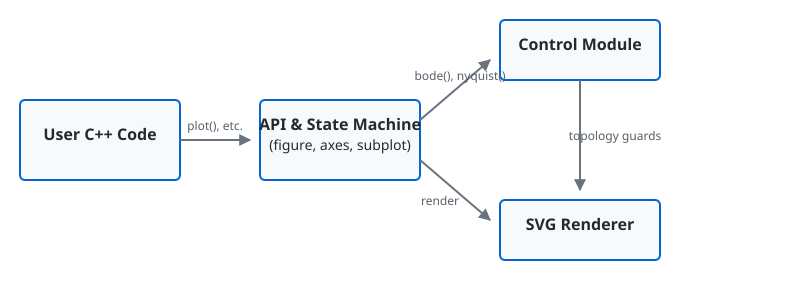
\includegraphics[width=0.85\linewidth]{../figures/fig_architecture.png}
    \caption{The core architecture of \texttt{CppPlot}. User C++ simulation code interacts exclusively through the matplotlib-inspired API layer. Domain-specific modules (e.g., Nyquist topology guards) process mathematical anomalies before pushing layout commands to the standalone SVG Renderer.}
    \label{fig:arch}
\end{figure}

\textbf{API layer.} The public API is deliberately modelled on matplotlib's pyplot interface. Format strings (\texttt{"b-o"}, \texttt{"r--"}, \texttt{"k:"}) control color, line style, and marker simultaneously. An \texttt{opts()} helper wraps \texttt{std::initializer\_list} into a convenient key-value map, preserving type safety while matching the visual style of matplotlib's \texttt{kwargs}.

\textbf{SVG backend.} All rendering is performed by a lightweight, self-contained SVG writer. The library produces standards-compliant SVG 1.1 output that renders identically in any modern browser, vector editor, and LaTeX workflow. Because SVG is XML-based text, the output is human-readable, diff-friendly, and version-control–compatible.

\textbf{Layout system.} \texttt{CppPlot} implements three complementary layout mechanisms: a MATLAB-style \texttt{subplot(rows, cols, index)} call; a \texttt{GridSpec} object with configurable width and height ratios and spacing; and free-form placement via \texttt{add\_axes(left, bottom, width, height)} in normalized figure coordinates. Cell spanning via \texttt{subplot\_span} and floating inset axes via \texttt{inset\_axes} are also supported.

\subsection{CppNB: Interactive Execution Environment}
\texttt{CppNB} provides a Jupyter-style interactive execution model tailored natively for C++. Unlike traditional REPLs (Read-Eval-Print Loops) that rely on interpreter abstractions like Cling, \texttt{CppNB} operates on a chunked compilation paradigm. Each \textit{code cell} in a \texttt{.cppnb} (or Markdown) notebook acts as a standalone C++ modification scope.

\textbf{Execution Pipeline.} When a cell is executed, an automated backend extracts the code, merges it with persistent global state and headers, and invokes the host \texttt{C++ compiler} in the background. The resulting binary is executed, and \texttt{CppNB} dynamically captures the \texttt{stdout} streams and natively generated SVG visualization assets.

\textbf{Inline Rendering.} The captured text output and SVG elements are streamed back to a Quarto-based \cite{Allaire2022} or HTML frontend, rendering a continuous visual report. Figure~\ref{fig:cppnb} demonstrates this workflow: the developer writes control-systems logic and plot commands in pure C++, and the resultant response graphs are immediately rendered inline directly below the execution cell. 

\begin{figure}[ht]
    \centering
    \includegraphics[width=\linewidth]{../figures/fig_cppnb_interface.png}
    \caption{The \texttt{CppNB} interactive interface. Code cells execute natively compiled C++ and immediately render the \texttt{CppPlot} SVG outputs inline, creating a seamless REPL-like experience for physical simulation.}
    \label{fig:cppnb}
\end{figure} 

\section{Feature Showcase}
\label{sec:features}

\subsection{General Scientific Plotting}
The library supports general-purpose scientific plotting (line, scatter, histogram, bar chart, error bars, fill-between, log-scale axes, multi-panel subplots). The \texttt{fill\_between} function is particularly useful for visualising uncertainty regions and confidence intervals in simulation results:

\begin{lstlisting}
auto x = linspace(0.0, 10.0, 200);
std::vector<double> y_mean, y_upper, y_lower;
for (double xi : x) {
    double v = std::sin(xi);
    y_mean.push_back(v);
    y_upper.push_back(v + 0.3 * std::exp(-0.1 * xi));
    y_lower.push_back(v - 0.3 * std::exp(-0.1 * xi));
}
figure(800, 450);
fill_between(x, y_lower, y_upper, opts({{"color","royalblue"},{"alpha","0.25"}}));
plot(x, y_mean, "b-", opts({{"linewidth","2"},{"label","Mean"}}));
title("Signal with Decaying Confidence Interval");
legend(true); savefig("confidence_band.svg");
\end{lstlisting}

\subsection{Control Systems: Frequency and Time Domain}
The control-systems module implements every major analysis plot used in classical and modern control design, following conventions compatible with Python Control \cite{Fuller2021} and standard textbooks \cite{Ogata2010, Franklin2019}.

\textbf{Bode plot.} Magnitude and phase are computed in user code and passed to the standard \texttt{plot} and \texttt{subplot} functions, giving full control over frequency range, annotation, and styling:

\begin{lstlisting}
double wn = 10.0, zeta = 0.3;
auto w = logspace(-1, 3, 500);
std::vector<double> mag_dB, phase_deg;
for (double wi : w) {
    std::complex<double> s(0, wi);
    auto H = (wn*wn) / (s*s + 2*zeta*wn*s + wn*wn);
    mag_dB.push_back(20.0 * std::log10(std::abs(H)));
    phase_deg.push_back(std::arg(H) * 180.0 / M_PI);
}
figure(800, 600);
subplot(2, 1, 1);
plot(w, mag_dB, "b-", opts({{"linewidth","2"}}));
xscale("log"); ylabel("Magnitude (dB)"); grid(true);
title("Bode Plot");

subplot(2, 1, 2);
plot(w, phase_deg, "b-", opts({{"linewidth","2"}}));
xscale("log"); xlabel("Frequency (rad/s)");
ylabel("Phase (deg)"); grid(true);
savefig("bode.svg");
\end{lstlisting}

\textbf{Integrator Bounding in Frequency Plots.} A common algorithmic challenge when generating automated Nyquist plots for systems containing integrators---i.e., open-loop transfer functions of the form $L(s) = N(s) / (s^k D(s))$---is the asymptotic magnitude explosion as $\omega \to 0^+$. Along the mapping of the Nyquist contour $s = r e^{j\theta}$ as $r \to 0$, the magnitude approaches infinity, $|L(s)| \approx |N(0)| / (r^k |D(0)|) \to \infty$, while the phase sweeps monotonically by $k \times 180^\circ$. This infinite topological span inherently dwarfs the critical $(-1, 0)$ stability region when plotted naively.

To resolve this, \texttt{CppPlot} implements a topology-aware bounding layer that intercepts unbounded coordinates. Rather than plotting the unbounded domain directly, the engine computes a constrained subset of the frequency response:
\begin{equation}
    \mathcal{P} = \left\{ L(j\omega) \mid \omega \in \Omega \right\} \cap \left\{ z \in \mathbb{C} \mid |z| \le M_{\max} \right\}
\end{equation}
The saturation radius $M_{\max}$ is algorithmically clamped relative to the phase crossover frequency $\omega_{pc}$, explicitly ensuring that the bounding-box $[\min \mathrm{Re}, \max \mathrm{Re}] \times [\min \mathrm{Im}, \max \mathrm{Im}]$ isolates the critical point $(-1, 0)$ and its surrounding margins, removing the need for manual axis rescaling by the user.

\subsection{Advanced Nonlinear Control}
This module constitutes the most distinctive contribution of \texttt{CppPlot} relative to other C++ plotting libraries. It provides visualization support for research-level nonlinear control algorithms, enabling figures that would previously have required MATLAB or Python scripts to be generated directly from the simulation source code.

\textbf{Sliding Mode Control variants.} The library includes example simulations and plot templates for Standard SMC, Super-Twisting SMC \cite{Levant1993}, Integral SMC, and combinations thereof. Figure generation follows the same pattern: numerically integrate the closed-loop ODE in C++, accumulate trajectory data, and call \texttt{CppPlot}.

\textbf{Control Barrier Functions (CBF).} Safety-critical control is an active research area \cite{Ames2019}. \texttt{CppPlot} provides facilities to visualise the state trajectory relative to a barrier boundary, the barrier function value over time, and the safety constraint margin.

\textbf{Fixed-Time Stabilization.} Fixed-time convergence controllers \cite{Polyakov2012} guarantee convergence within a bounded time independent of initial conditions. \texttt{CppPlot} can overlay multiple trajectories starting from different initial conditions, visually demonstrating this property.

\section{Real-Time Optimization and Embedded MPC}
\label{sec:mpc}

\subsection{ADMM Formulation}
Model Predictive Control poses the regulation task as a constrained Quadratic Program (QP) solved iteratively online:
\begin{equation}
    \min_{U} \tfrac{1}{2} U^\top H U + g(x_0)^\top U \quad \text{s.t.} \quad U \in \mathcal{C} = \{U \mid \mathbf{lb} \le U \le \mathbf{ub}\}
\end{equation}
where the Hessian $H = \Gamma^\top \bar{Q} \Gamma + \bar{R}$ is dense and invariant, and the gradient vector $g = \Gamma^\top \bar{Q}\Phi x_0$ depends strictly on the current state. To optimize this within embedded hard real-time constraints, we decoupled the objective and the set $\mathcal{C}$ utilizing the Alternating Direction Method of Multipliers (ADMM). 

The algorithm introduces an auxiliary formulation with constraints $U - Z = 0$ over learning states $Z \in \mathcal{C}$. The Augmented Lagrangian is then minimized iteratively:
\begin{align}
    U^{k+1} &= (H + \rho I)^{-1}(\rho Z^k - Y^k - g) \label{eq:admm_u}\\
    Z^{k+1} &= \Pi_{\mathcal{C}}\left( U^{k+1} + Y^k/\rho \right) \label{eq:admm_z}\\
    Y^{k+1} &= Y^k + \rho(U^{k+1} - Z^{k+1}) \label{eq:admm_y}
\end{align}
where $Y$ represents the dual variable (multipliers), $\rho > 0$ the penalty parameter, and $\Pi_{\mathcal{C}}$ the Euclidean projection operator onto the inequality bounds. The linear system step \eqref{eq:admm_u} avoids dense inversion via static Cholesky pre-factorization.

\subsection{Benchmarking on Embedded Scenarios}
Validating such solvers necessitates complex visual diagnostics for convergence—defined by the primal residual and dual residual. \texttt{CppPlot} natively generates real-time optimization diagnostics to debug and validate these embedded solvers without any data export. 

Because solve times span three orders of magnitude (0.29 $\mu$s to 375 $\mu$s), a logarithmic y-axis is essential for legibility. The \texttt{boxplot()} capability renders full IQR, whiskers, and outliers natively under \texttt{yscale("log")}:

\begin{lstlisting}
boxplot(all_times, positions, opts({{"widths","0.6"}}));
yscale("log");
axhline(10000.0, opts({{"color","red"},{"linestyle","--"},
                       {"label","10 ms deadline"}}));
\end{lstlisting}

Table~\ref{tab:bench} summarises benchmark results obtained for a 10-dimensional MPC QP ($N=10$ horizon) across three scenarios (60 timing repetitions, 20 initial conditions per scenario, x86-64, GCC \texttt{-O3}). Figure~\ref{fig:timing} visualizes this data, showing the true log-scale boxplot. Figure~\ref{fig:tradeoff} renders a Time-Accuracy Pareto scatter comparing ADMM and classical Projected Gradient Descent (PGD).

\begin{table}[ht]
\centering
\caption{Median and P95 solve time ($\mu$s), $N=10$, GCC \texttt{-O3}. ADMM cold-start Conv=0\% on S2 is due to a fully-active constraint set, requiring ADMM tuning or warm-start. WCET worst case: 375 $\mu$s $\ll$ 10 ms deadline.}
\label{tab:bench}
\resizebox{\linewidth}{!}{
\begin{tabular}{@{}lcccc@{}}
\toprule
Solver & S1 Easy (Med/P95) & S2 Medium (Med/P95) & S3 Hard (Med/P95) & Conv. S1/S2/S3 \\ 
\midrule
ADMM-cold ($\rho=1$) & 27.7 / 34.6 & 57.5 / 67.7 & 17.4 / 24.5 & 100\% / 0\% / 85\% \\
ADMM-tuned ($\rho^*$) & 130 / 149 & 262 / 300 & 35.4 / 48.0 & 100\% / 0\% / 100\% \\
\textbf{ADMM, warm-start} & \textbf{30.4 / 33.4} & \textbf{56.6 / 63.2} & \textbf{16.6 / 20.9} & 100\% / 0\% / 85\% \\
PGD (Barzilai-Borwein) & 29.3 / 32.5 & 200 / 244 & 132 / 168 & 100\% / 0\% / 0\% \\
CG-proj & 0.95 / 1.28 & 116 / 148 & 110 / 142 & 100\% / 15\% / 0\% \\
\textbf{Chol-Direct$^\dagger$} & \textbf{0.29 / 0.42} & \textbf{0.23 / 0.42} & \textbf{0.20 / 0.58} & 100\% / 100\% / 100\% \\
\bottomrule
\end{tabular}
}
\end{table}

\begin{figure}[ht]
    \centering
    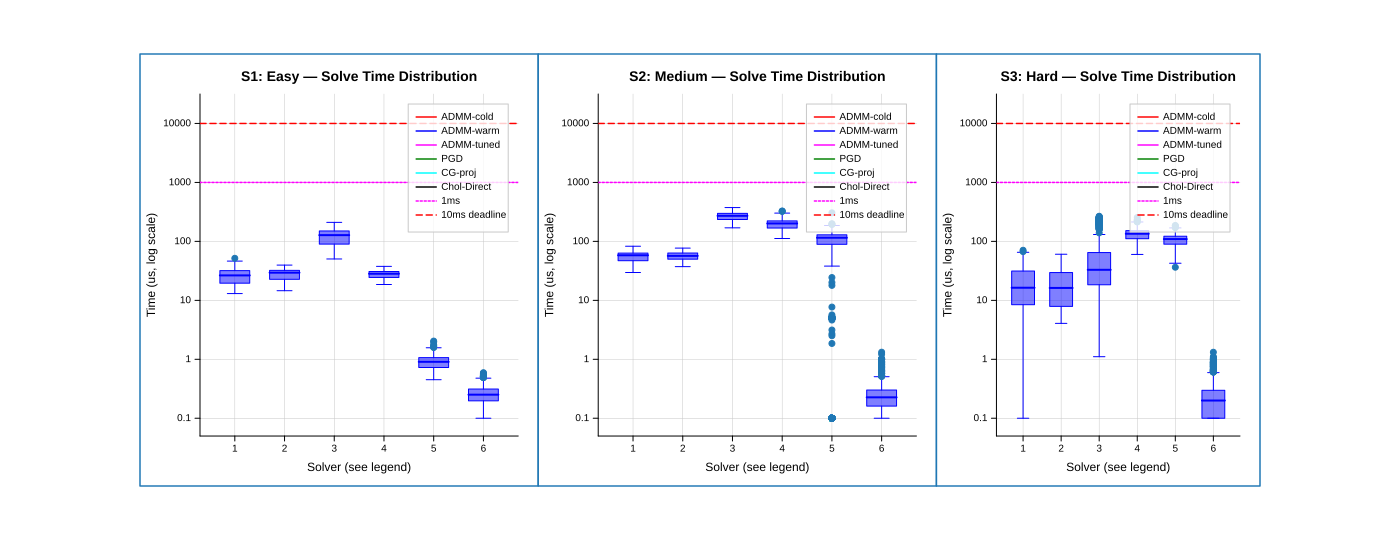
\includegraphics[width=\linewidth]{../figures/fig_bench_timing.png}
    \caption{Timing distributions for QP solvers across three MPC scenarios. All solvers are $\ge$26$\times$ below the 10 ms deadline. Outliers and IQR rendered natively by \texttt{boxplot()}.}
    \label{fig:timing}
\end{figure}

\begin{figure}[ht]
    \centering
    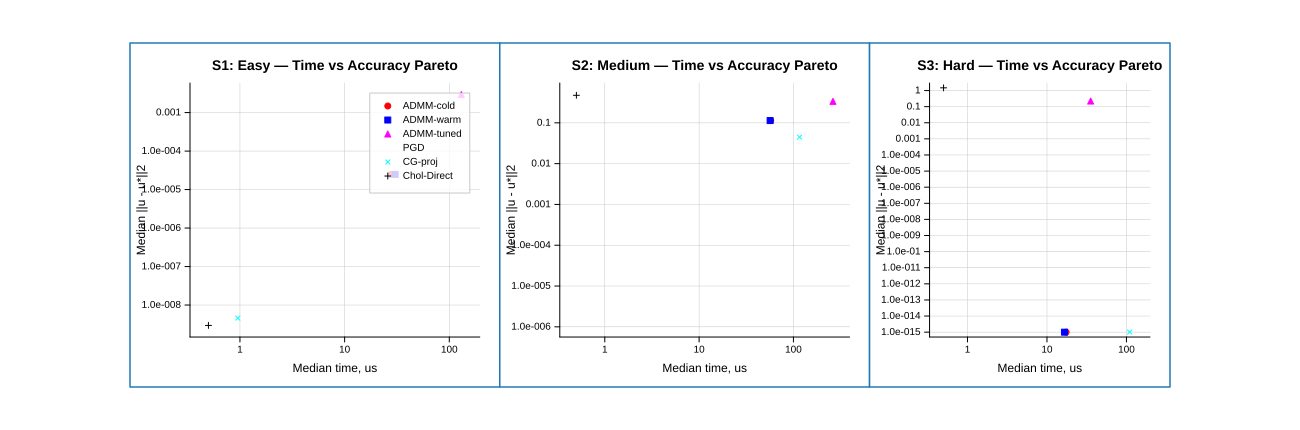
\includegraphics[width=\linewidth]{../figures/fig_bench_tradeoff.png}
    \caption{Time-accuracy Pareto scatter for the Hard scenario. Log-log axes generated natively via \texttt{xscale("log")} and \texttt{yscale("log")}.}
    \label{fig:tradeoff}
\end{figure}

\section{Reproducibility}
A central design goal of the toolkit is enabling fully reproducible computational figures. Every figure in the repository can be regenerated from source with three commands: \texttt{mkdir build \&\& cd build}, \texttt{cmake .. \&\& cmake --build .}, and \texttt{ctest}. No additional runtime or package manager is required beyond a C++14 compiler and CMake. This property is particularly significant for engineering research, where the ability to audit, modify, and re-run simulations from their original source code is a key component of scientific integrity \cite{Sandve2013, Peng2011}.

\section{Developer Experience and Methodology}

\subsection{Integration}
\texttt{CppPlot} supports integration via simple Header Copy, CMake \texttt{add\_subdirectory}, or CMake \texttt{FetchContent} (recommended for reproducible builds). It is verified to compile on GCC 6.3+, Clang 5.0+, and MSVC 2017+ across Linux, macOS, and Windows.

\subsection{AI-Assisted Development Methodology}
The core implementations of both libraries were substantially generated and refined through an \textit{agentic AI} development workflow, in which large language models (LLMs) served as code-generation and refactoring agents guided by a human architect. This workflow raises an interesting methodological question: can agentic AI systems generate library-quality scientific software? The repositories presented here represent a positive data point—the generated code passes a cross-platform CMake test suite, produces visually correct SVG output across all supported compilers, and implements domain-correct control-systems algorithms.

The benchmark file \texttt{benchmark\_qp\_solvers\_V7.cpp} (the final of seven iterative versions) illustrates this workflow. Agentic review passes identified 19 bugs across seven versions, categorised into logic errors (e.g., critical reference-solver misconfigurations) and timing-measurement errors (detectable only by running on hardware, including clock-granularity failures and integer-truncation). Each bug was corrected with a targeted patch, demonstrating that correctness emerges from iterative AI-assisted inspection rather than from a single generation step.

\section{Conclusions}
\label{sec:conclusions}
The proposed toolchain addresses a long-standing workflow gap in C++ scientific computing. By integrating high-quality SVG generation and interactive notebook capabilities directly into native C++, researchers and engineers gain the ability to validate complex control and optimization algorithms robustly in real-time. Future work involves WebAssembly integration for dynamic browser-based interactivity and enhanced 3D plotting capabilities.

\section*{Acknowledgements}
The control-systems domain knowledge embedded in the library draws on foundational texts by Ogata \cite{Ogata2010}, Franklin et al. \cite{Franklin2019}, and Slotine and Li \cite{Slotine1991}. Inspiration for the API is acknowledged to Hunter et al. \cite{Hunter2007}.

\bibliographystyle{elsarticle-num}
\bibliography{references}

\end{document}
